\begin{table}[htbp]
	\centering
	\begin{tabular}{|l|l|}
		\hline
		\textbf{Description} & \textbf{Results} \\ \hline
		Keywords Plus & 1695 \\ \hline
		Author's Keywords & 2404 \\ \hline
	\end{tabular}
	\caption{Palabras clave contenidas en los documentos}
	\label{tb:keywords}
\end{table}

\subsection{Redes de palabras clave}

\begin{figure}[ht]
	\centering
	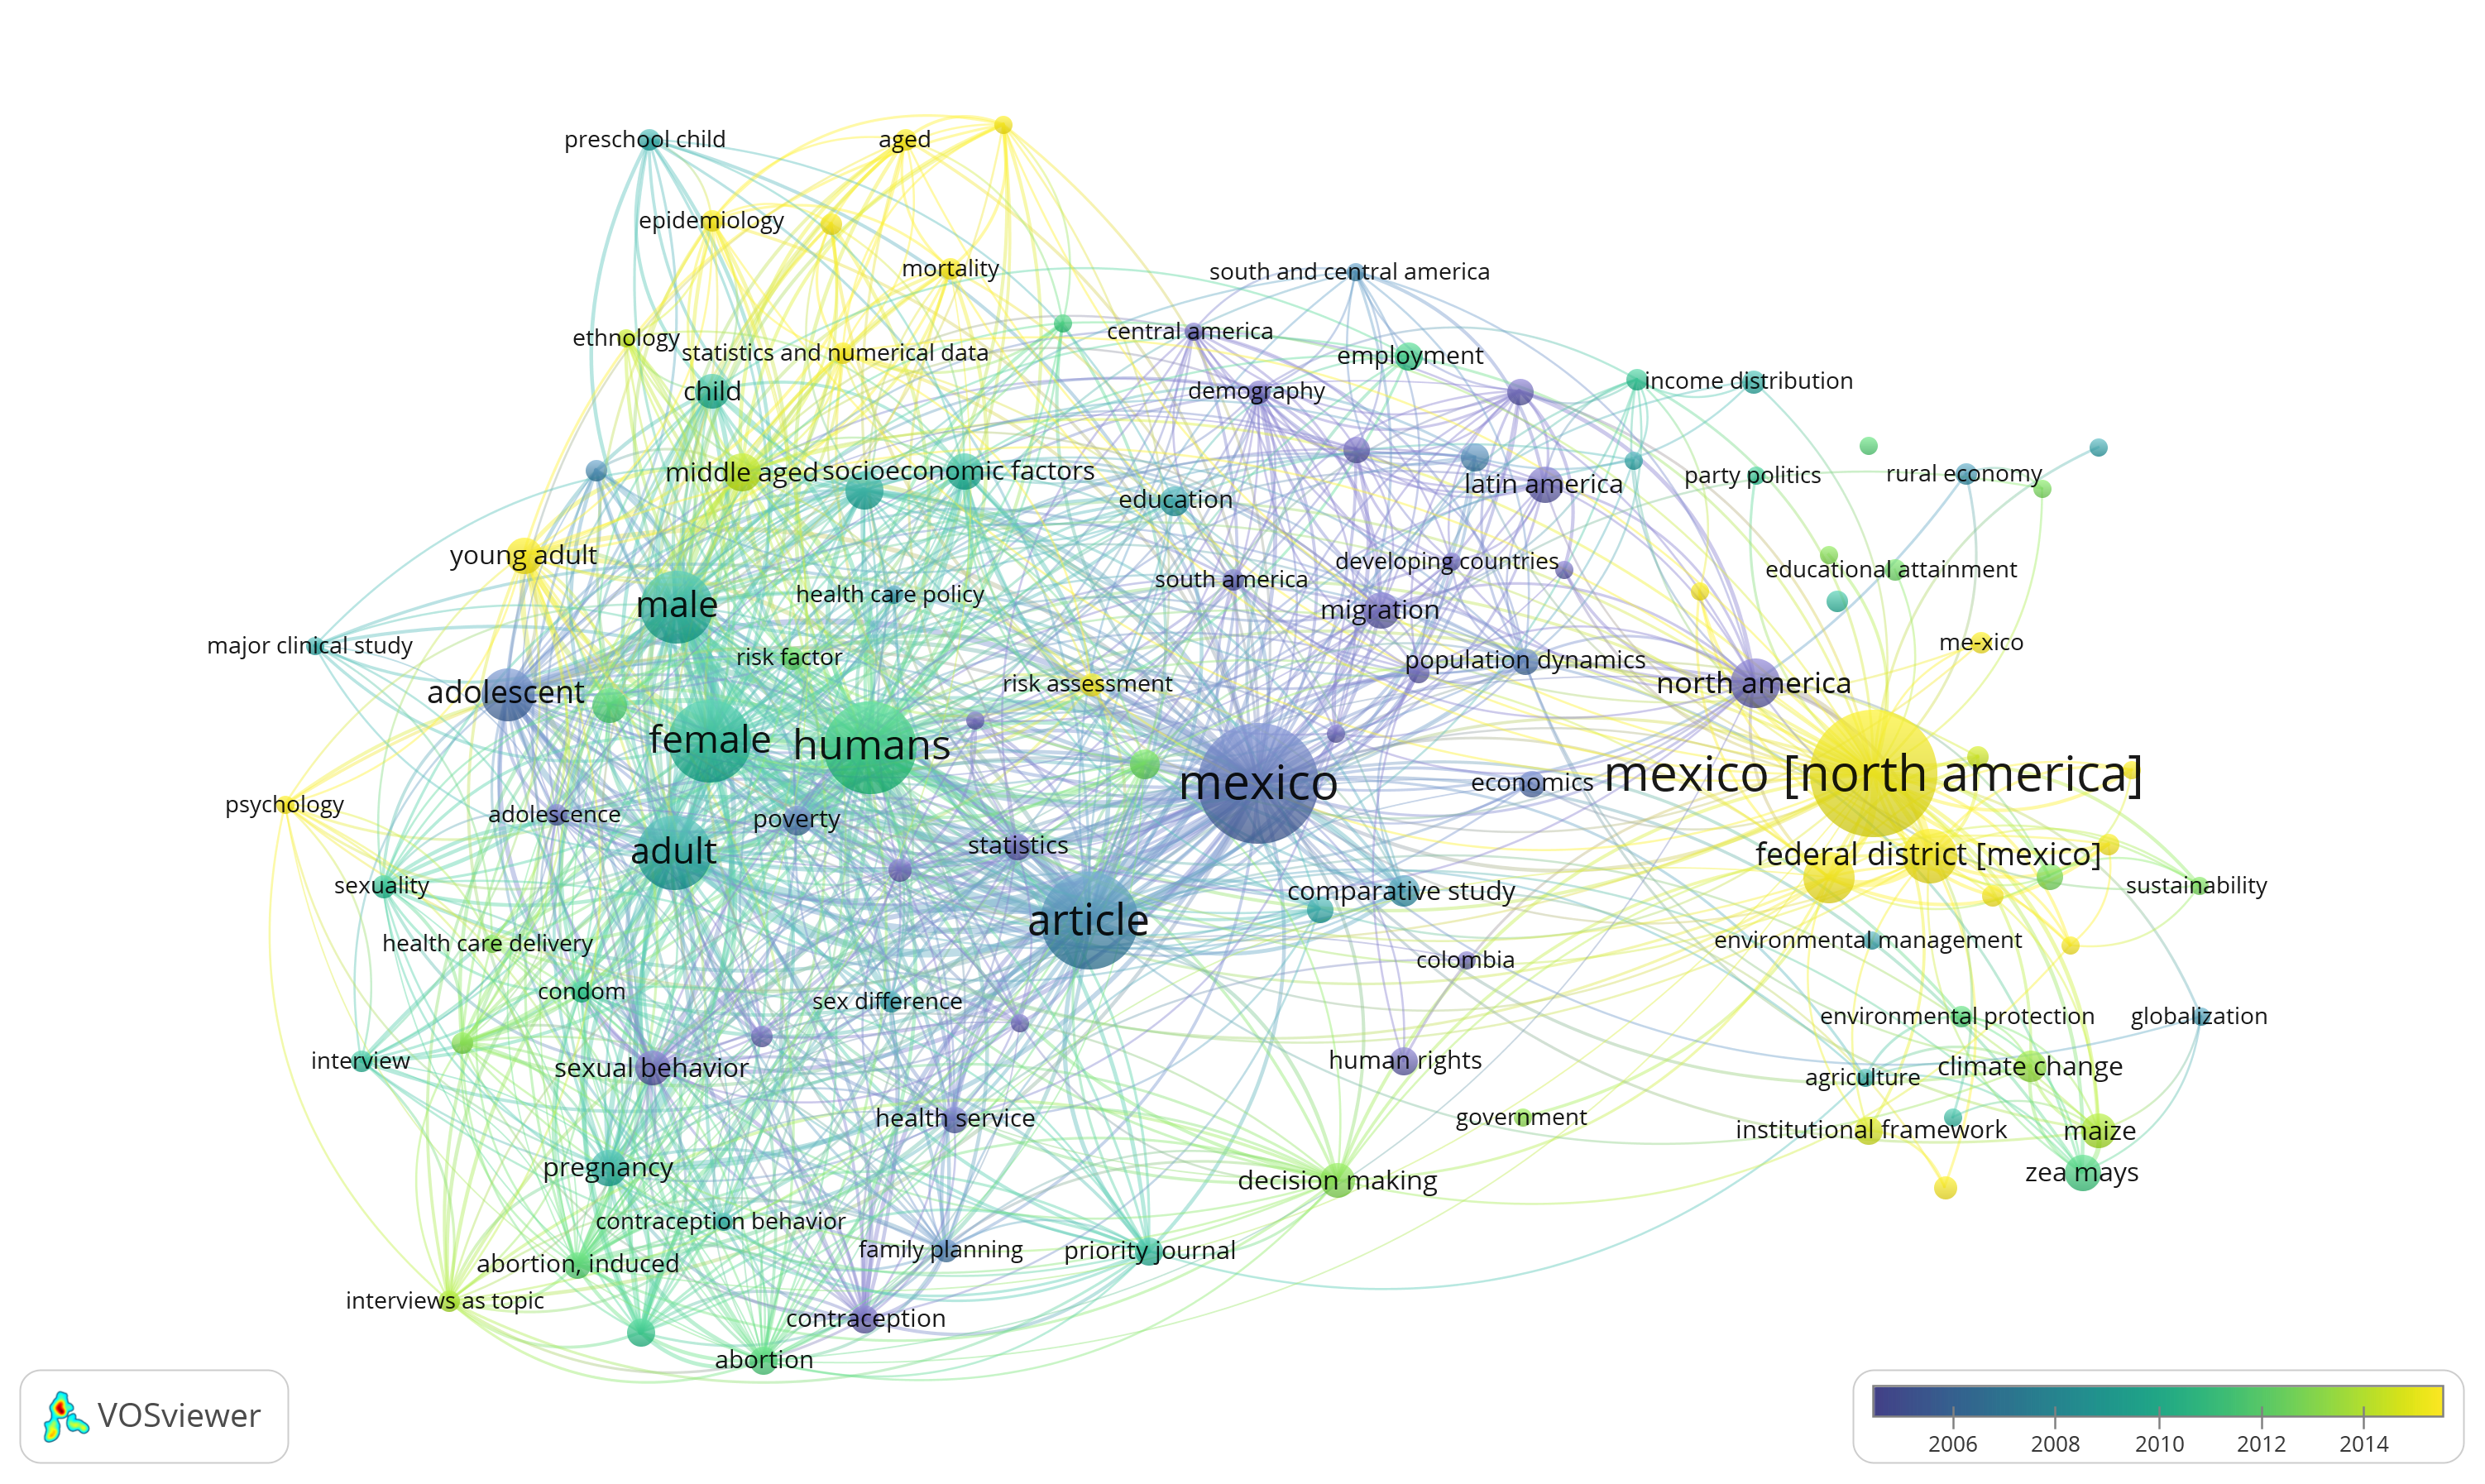
\includegraphics[width=\textwidth]{imagenes/net_kw_tiempo.png}
	\caption{Evolución temporal de la red de palabras clave.}
	\label{fig:ckw_tiempo}   
\end{figure}

\begin{figure}[ht]
	\centering
	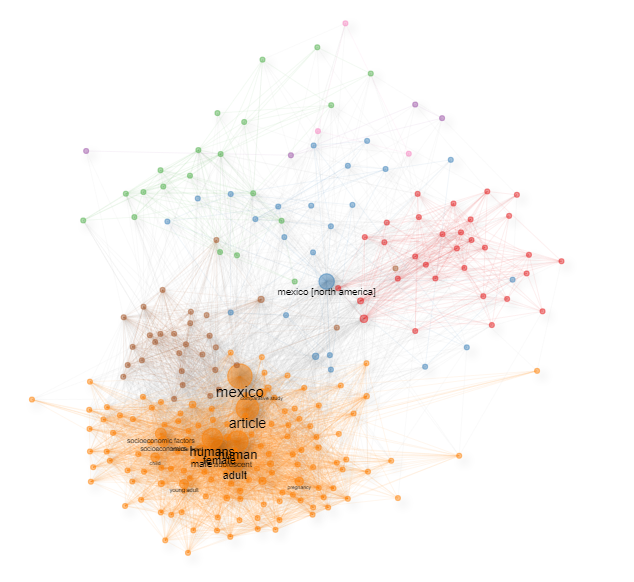
\includegraphics[width=\textwidth]{imagenes/net_kw_comunidades.png}
	\caption{Comunidades detectadas en la red de palabras clave.}
	\label{fig:kw_comunidades}   
\end{figure}
\begin{figure}[ht]
	\centering
	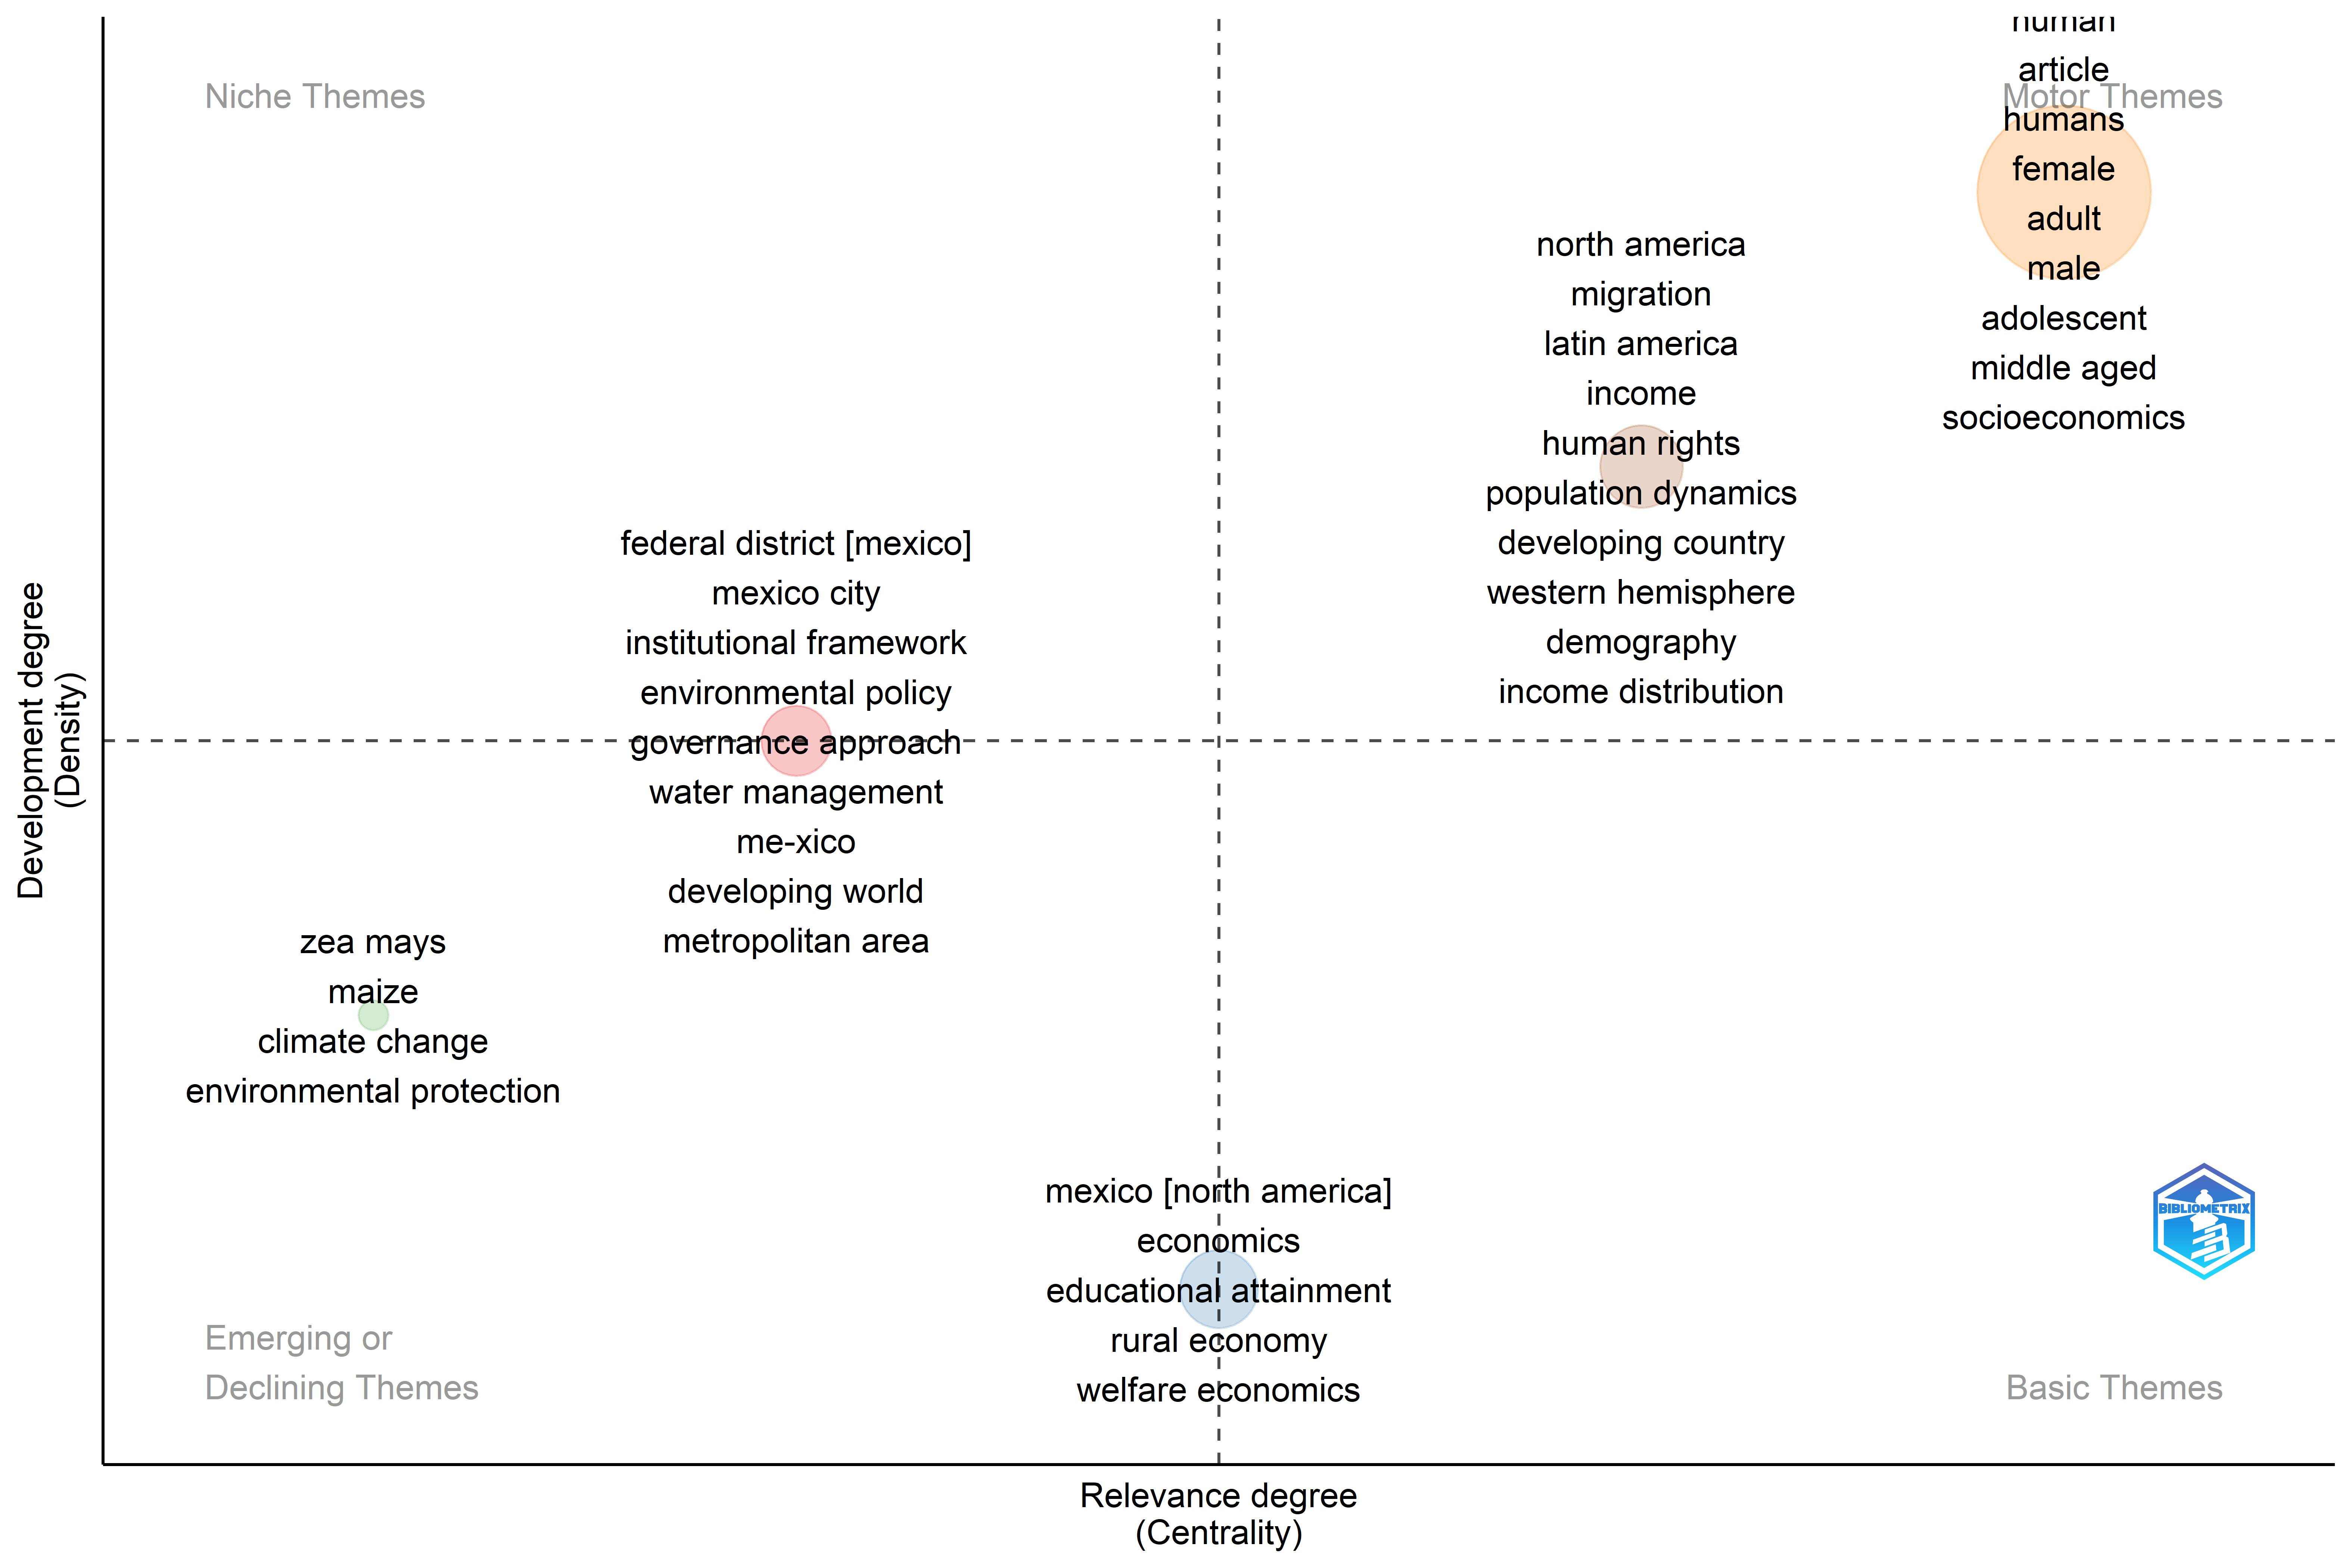
\includegraphics[width=\textwidth]{imagenes/mapa_tematico.png}
	\caption{Mapa temático basado en las comunidades de la red de palabras clave.}
	\label{fig:kw_comunidades}   
\end{figure}


\begin{figure}[ht]
	\centering
	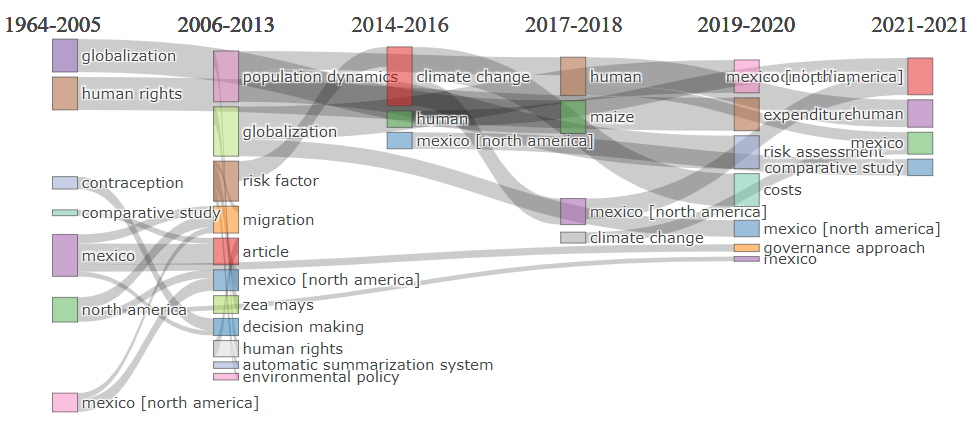
\includegraphics[width=\textwidth]{imagenes/evolucion_tematica.png}
	\caption{Evolución temática basada en el uso de palabras clave.}
	\label{fig:tematic_map}   
\end{figure}
